\chapter{Implementacija i korisničko sučelje}
		
		\section{Korištene tehnologije i alati}
		
			%\textbf{\textit{dio 2. revizije}}\\
			
            Komunikacija u timu realizirana je korištenjem aplikacije\underline{ Discord}\footnote{\url{https://discord.com/}},\underline{ MicrosoftTeams}\footnote{\url{https://www.microsoft.com/en-us/microsoft-365/microsoft-teams}} i \underline{WhatsApp}\footnote{\url{https://www.whatsapp.com/}}. Za izradu UML dijagrama korišten je alat \underline{Astah Professional}\footnote{\url{https://astah.net/}}, a kao sustav za upravljanje izvornim kodom \underline{Git}\footnote{\url{https://git-scm.com/}}. Udaljeni repozitorij projekta je dostupan na web platformi \underline{GitLab}\footnote{\url{https://about.gitlab.com/}}.
            Kao razvojno okruženje korišteni su \underline{IntelliJ}
            \footnote{\url{https://www.jetbrains.com/idea/}} - integrirano razvojno okruženje (IDE) tvrtke JetBrains.
            \underline{Spring Tool Suite}
            \footnote{\url{https://spring.io/tools}} (Eclipse) - integrirano razvojno okruženje namijenjeno za razvoj aplikacija koje koriste Spring kao radni okvir te \underline{VSCode}\footnote{\url{https://code.visualstudio.com/}} - integrirano razvojno okruženje pogodno za razvoj frontend-a.
            
            Aplikacija je napisana koristeći  radni
            okvir \underline{Spring Boot}\footnote{\url{https://spring.io/projects/spring-boot}} i jezik \underline{Javu}\footnote{\url{https://www.java.com/}} za
            izradu \emph{backenda} te \underline{React}\footnote{\url{https://reactjs.org/}} i jezik \underline{JavaScript}\footnote{\url{https://www.javascript.com/}} za izradu \emph{frontenda}.
            Spring Boot je open-source Javin radni okvir koji omogućuje izgradnju mikro servisa. Sam Spring Boot dolazi s već predkonfiguriranim značajkama koje programerima omogućuju konvencijonalnost te mogućnost pokretanja aplikacije bez dodatnog posla. 
            React, također poznat kao React.js ili ReactJS, je biblioteka u JavaScriptu za izgradnju korisničkih
            sučelja. Složene aplikacije u React-u obično zahtijevaju korištenje dodatnih biblioteka za interakciju s API-jem.
            
            Baza podataka i aplikacija se nalaze na poslužitelju \underline{Heroku}
            \footnote{\url{https://www.heroku.com/}}.
            
        
\newpage 

\begin{comment}   
        \section{Ispitivanje programskog rješenja}
			
			\textbf{\textit{dio 2. revizije}}
			
			Svi testovi izvršeni su pomoću Junit i Selenium. Ispitivanje se radilo po obrascima uporabe kako bi
            se provjerila osnovna funkcionalnost sustava, ali i nasumičnim kretanjima po aplikaciji
            kako bi se pronašle neočekivane greške  ili nepredvidena ponašanja.
            Svaki dio sustava je ispitan, no zbog jednostavnosti u dokumentaciji će biti prikazan
            samo dio ispitivanja. Prikazivanje ispitivanja UC?, UC?, UC?,UC?, UC? i UC?.
            
\end{comment}

		    \section{Ispitivanje programskog rješenja}
\begin{comment}
			\textbf{\textit{dio 2. revizije}}\\
			
			 \textit{U ovom poglavlju je potrebno opisati provedbu ispitivanja implementiranih funkcionalnosti na razini komponenti i na razini cijelog sustava s prikazom odabranih ispitnih slučajeva. Studenti trebaju ispitati temeljnu funkcionalnost i rubne uvjete.}
\end{comment} 
        
%\begin{comment}
        \subsection{Ispitivanje komponenti}
		    
	
    
			\textit { Provesli smo  ispitivanje-unit testing nad razredima koji implementiraju temeljne funkcionalnosti, a to su User i Request. Ispitali smo njihovih 7 metoda te njihove redovne slučajeve, rubne slučajeve i one koji izazivaju pogrešku.Pri testiranju su korišteni pripremljeni podatci u bazi koji se unose automatski pri svakom pokretanju testa. }
			
			\medskip
			
			\noindent \textbf{Ispitni slučaj 1: Testiranje funkcionalnosti metode updateUser()}\\
			
			\medskip
            \noindent\textbf{Ulaz:}
            \begin{packed_enum}
            \item vrijednosti UserDTO
            \item Id korisnika čiji se profil uređuje
            \item User principal
            \end{packed_enum}
            
            \noindent\textbf{Očekivani rezultat:}
            \begin{packed_enum}
            \item uređeni user
            \item pripadajuća pogreška
            \end{packed_enum}
            
            \noindent \text
            Rezultat: Očekivani rezultat je zadovoljen, aplikacija je prošla sve testove \\
            
            \begin{figure}[H]
                 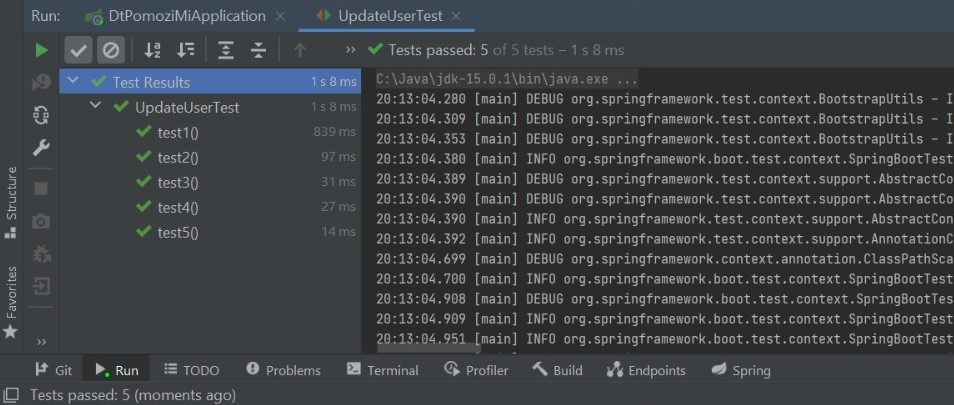
\includegraphics[width=\textwidth, height=\textheight, keepaspectratio]{slike/UpdateUserTest.jpeg}
                \centering
                \caption{UpdateUserTest()}
            \end{figure}
            
            \noindent \textbf{Kod unit testa: }
            
            \begin{verbatim}
			package NULL.DTPomoziMi.service.impl;

import static org.junit.jupiter.api.Assertions.assertEquals;
import static org.junit.jupiter.api.Assertions.assertThrows;

import org.junit.jupiter.api.Test;
import org.springframework.beans.factory.annotation.Autowired;
import org.springframework.boot.test.context.SpringBootTest;
import org.springframework.dao.DataIntegrityViolationException;
import org.springframework.security.test.context.support.WithUserDetails;
import org.springframework.test.context.ActiveProfiles;

import NULL.DTPomoziMi.exception.IllegalAccessException;
import NULL.DTPomoziMi.model.User;
import NULL.DTPomoziMi.security.UserPrincipal;
import NULL.DTPomoziMi.service.UserService;
import NULL.DTPomoziMi.util.UserPrincipalGetter;
import NULL.DTPomoziMi.web.DTO.UserDTO;
import NULL.DTPomoziMi.web.assemblers.UserDTOModelAssembler;

@SpringBootTest
@ActiveProfiles("dev")
public class UpdateUserTest {

	@Autowired
	private UserService service;

	@Autowired
	private UserDTOModelAssembler assembler;

	private UserPrincipal principal;

	private UserDTO userDTO;

	public void setup() { userDTO = assembler.toModel(service.fetch(11)); }

	//korisnik ima pristup uredivanju profila
	@Test
	@WithUserDetails(value = "marija.orec@gmail.com", 
	userDetailsServiceBeanName = "myUserDetailsService")
	public void test1() {
		setup();
		principal = UserPrincipalGetter.getPrincipal();

		userDTO.setEmail("bananko@gmail.com");
		userDTO.setFirstName("Janko");
		userDTO.setLastName("bananko");
		userDTO.setPicture("aaa");

		service.updateUser(userDTO, 11, principal);

		User user = service.fetch(11);

		assertEquals(user.getEmail(), userDTO.getEmail());
		assertEquals(user.getFirstName(), userDTO.getFirstName());
		assertEquals(user.getLastName(), userDTO.getLastName());
		assertEquals(user.getPicture(), userDTO.getPicture());
		assertEquals(user.getIdUser(), userDTO.getIdUser());
	}

	// korisnik je postavio već postojeći email
	@Test
	@WithUserDetails(value = "bananko@gmail.com", 
	userDetailsServiceBeanName = "myUserDetailsService")
	public void test2() {
		setup();
		principal = UserPrincipalGetter.getPrincipal();

		userDTO.setEmail("matea.lipovac@gmail.com");
		assertThrows(DataIntegrityViolationException.class, 
		() -> service.updateUser(userDTO, 11, principal));
	}

	//korisnik nema pristup uredivanju profila
	@Test
	@WithUserDetails(value = "matea.lipovac@gmail.com",
	userDetailsServiceBeanName = "myUserDetailsService")
	public void test3() {
		setup();
		principal = UserPrincipalGetter.getPrincipal();
		assertThrows(IllegalAccessException.class,
		() -> service.updateUser(userDTO, 11, principal));
	}

	//userDTO i id se ne poklapaju
	@Test
	@WithUserDetails(value = "bananko@gmail.com",
	userDetailsServiceBeanName = "myUserDetailsService")
	public void test4() {
		setup();
		principal = UserPrincipalGetter.getPrincipal();
		assertThrows(IllegalArgumentException.class,
		() -> service.updateUser(userDTO, 3, principal));
	}

	//neprijavljen korisnik
	@Test
	public void test5() {
		principal = UserPrincipalGetter.getPrincipal();
		assertThrows(AuthenticationCredentialsNotFoundException.class, 
		() -> service.updateUser(userDTO, 11, principal));
	}
}
            \end{verbatim}
			
			
				\medskip
			
			\noindent \textbf{Ispitni sličaj 2: Testiranje funkcionalnosti metode updateRequest()}\\
			
			\medskip
            \noindent\textbf{Ulaz:}
            \begin{packed_enum}
            \item id zahtjeva koji se uređuje
            \item vrijednosti RequestDTO
            \item User principal
            \end{packed_enum}
            
            \noindent\textbf{Očekivani rezultat:}
            \begin{packed_enum}
            \item uređeni zahtjev
            \item pripadajuća pogreška
            \end{packed_enum}
            
            \noindent \text
            Rezultat: Očekivani rezultat je zadovoljen, aplikacija je prošla sve testove \\
            
            \begin{figure}[H]
                 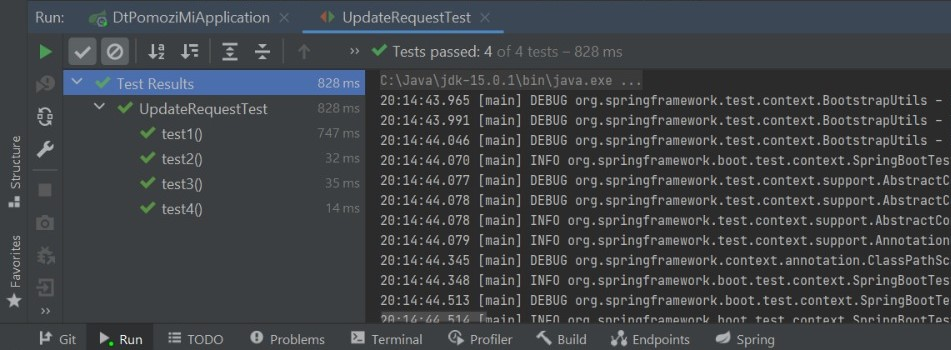
\includegraphics[width=\textwidth, height=\textheight, keepaspectratio]{slike/UpdateRequestTest.jpeg}
                \centering
                \caption{UpdateRequestTest()}
            \end{figure}
            
            \noindent \textbf{Kod unit testa: }
            \begin{verbatim}
            package NULL.DTPomoziMi.service.impl;

import static org.junit.jupiter.api.Assertions.assertEquals;
import static org.junit.jupiter.api.Assertions.assertNotEquals;
import static org.junit.jupiter.api.Assertions.assertNotNull;
import static org.junit.jupiter.api.Assertions.assertNull;
import static org.junit.jupiter.api.Assertions.assertThrows;

import java.time.LocalDateTime;

import org.junit.jupiter.api.Test;
import org.springframework.beans.factory.annotation.Autowired;
import org.springframework.boot.test.context.SpringBootTest;
import org.springframework.security.authentication.
AuthenticationCredentialsNotFoundException;
import org.springframework.security.test.context.support.WithUserDetails;
import org.springframework.test.context.ActiveProfiles;

import NULL.DTPomoziMi.exception.IllegalAccessException;
import NULL.DTPomoziMi.model.Request;
import NULL.DTPomoziMi.model.RequestStatus;
import NULL.DTPomoziMi.security.UserPrincipal;
import NULL.DTPomoziMi.util.UserPrincipalGetter;
import NULL.DTPomoziMi.web.DTO.RequestDTO;
import NULL.DTPomoziMi.web.assemblers.RequestDTOAssembler;

@SpringBootTest
@ActiveProfiles("dev")
public class UpdateRequestTest {
	@Autowired
	private RequestServiceImpl service;

	@Autowired
	private RequestDTOAssembler assembler;

	private RequestDTO request;

	public void setup() { request = assembler.toModel(service.fetch(27)); }

	//uspjsan update
	@Test
	@WithUserDetails(value = "dominik.curic@gmail.com",
	userDetailsServiceBeanName = "myUserDetailsService")
	public void test1() {
		setup();
		UserPrincipal principal = UserPrincipalGetter.getPrincipal();

		final String phone = "091";
		final LocalDateTime ldt = LocalDateTime.of(2022, 1, 1, 1, 1, 1);
		final String desc = "abc";

		request.setDescription(desc);
		request.setPhone(phone);
		request.setTstmp(ldt);
		request.setLocation(null);
		request.setAuthor(null);
		request.setStatus(RequestStatus.FINALIZED);

		service.updateRequest(27, request, principal);
		Request updated = service.fetch(27);

		assertEquals(phone, updated.getPhone());
		assertEquals(ldt, updated.getTstmp());
		assertEquals(desc, updated.getDescription());
		assertNull(updated.getLocation());
		assertNotEquals(123L, updated.getIdRequest());
		assertNotNull(updated.getAuthor());
		assertNotEquals(RequestStatus.FINALIZED, updated.getIdRequest());

	}

	//id requesta i id reguestDTOa razliciti
	@Test
	@WithUserDetails(value = "dominik.curic@gmail.com",
	userDetailsServiceBeanName = "myUserDetailsService")
	public void test2() {
		setup();
		UserPrincipal principal = UserPrincipalGetter.getPrincipal();
		assertThrows(IllegalArgumentException.class, 
		() -> service.updateRequest(3, request, principal));
	}

	//nije autor
	@Test
	@WithUserDetails(value = "jan.rocek@gmail.com",
	userDetailsServiceBeanName = "myUserDetailsService")
	public void test3() {
		setup();
		UserPrincipal principal = UserPrincipalGetter.getPrincipal();
		assertThrows(IllegalAccessException.class,
		() -> service.updateRequest(27, request, principal));
	}

	//neprijavljen korisnik
	@Test
	public void test4() {
		UserPrincipal principal = UserPrincipalGetter.getPrincipal();
		assertThrows(AuthenticationCredentialsNotFoundException.class,
		() -> service.updateRequest(19, request, principal));
	}
}
		\end{verbatim}
			
			\medskip
			
			\noindent \textbf{Ispitni sličaj 3: Testiranje funkcionalnosti metode pickForExecution()}\\
			
			\medskip
            \noindent\textbf{Ulaz:}
            \begin{packed_enum}
            \item id zahtjeva koji se odabire
            \item User principal
            \end{packed_enum}
            
            \noindent\textbf{Očekivani rezultat:}
            \begin{packed_enum}
            \item zahtjev je u statusu izvrsavanja (executing)
            \item pripadajuća pogreška
            \end{packed_enum}
            
            \noindent \text
            Rezultat: Očekivani rezultat je zadovoljen, aplikacija je prošla sve testove \\
            
            \begin{figure}[H]
                 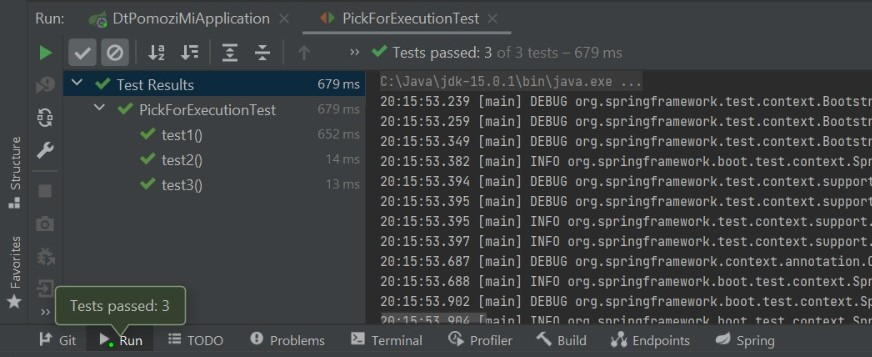
\includegraphics[width=\textwidth, height=\textheight, keepaspectratio]{slike/PickForExecutionTest.jpeg}
                \centering
                \caption{PickForExecutionTest()}
            \end{figure}
            
            \noindent \textbf{Kod unit testa: }
            \begin{verbatim}
			package NULL.DTPomoziMi.service.impl;

import static org.junit.jupiter.api.Assertions.assertEquals;
import static org.junit.jupiter.api.Assertions.assertThrows;

import org.junit.jupiter.api.Test;
import org.springframework.beans.factory.annotation.Autowired;
import org.springframework.boot.test.context.SpringBootTest;
import org.springframework.security.authentication.
AuthenticationCredentialsNotFoundException;
import org.springframework.security.test.context.support.WithUserDetails;
import org.springframework.test.context.ActiveProfiles;

import NULL.DTPomoziMi.exception.IllegalActionException;
import NULL.DTPomoziMi.model.RequestStatus;
import NULL.DTPomoziMi.security.UserPrincipal;
import NULL.DTPomoziMi.service.RequestService;
import NULL.DTPomoziMi.util.UserPrincipalGetter;

@SpringBootTest
@ActiveProfiles("dev")

public class PickForExecutionTest {
	@Autowired
	private RequestService service;

	//uspjesno odabrano izvrsavanje
	@Test
	@WithUserDetails(value = "iva.boksic@gmail.com",
	userDetailsServiceBeanName = "myUserDetailsService")
	public void test1() {
		UserPrincipal principal = UserPrincipalGetter.getPrincipal();
		service.pickForExecution(14, principal).getStatus();
		assertEquals(RequestStatus.EXECUTING, service.fetch(14).getStatus());
	}

	//neaktivan zahtjev
	@Test
	@WithUserDetails(value = "iva.boksic@gmail.com",
	userDetailsServiceBeanName = "myUserDetailsService")
	public void test2() {
		UserPrincipal principal = UserPrincipalGetter.getPrincipal();
		assertThrows(IllegalActionException.class, 
		() -> service.pickForExecution(24, principal));
	}

	//neprijavljen korisnik
	@Test
	public void test3() {
		UserPrincipal principal = UserPrincipalGetter.getPrincipal();
		assertThrows(AuthenticationCredentialsNotFoundException.class, 
		() -> service.deleteRequest(14, principal).getStatus());
	}
}
			\end{verbatim}
			
			\medskip
			
			\noindent \textbf{Ispitni sličaj 4: Testiranje funkcionalnosti metode getUserById()}\\
			
			\medskip
            \noindent\textbf{Ulaz:}
            \begin{packed_enum}
            \item id korisnika koji se dohvaća
            \item User principal
            \end{packed_enum}
            
            \noindent\textbf{Očekivani rezultat:}
            \begin{packed_enum}
            \item korisnik s traženim idom
            \item pripadajuća pogreška
            \end{packed_enum}
            
            \noindent \text
            Rezultat: Očekivani rezultat je zadovoljen, aplikacija je prošla sve testove \\
            
            \begin{figure}[H]
                 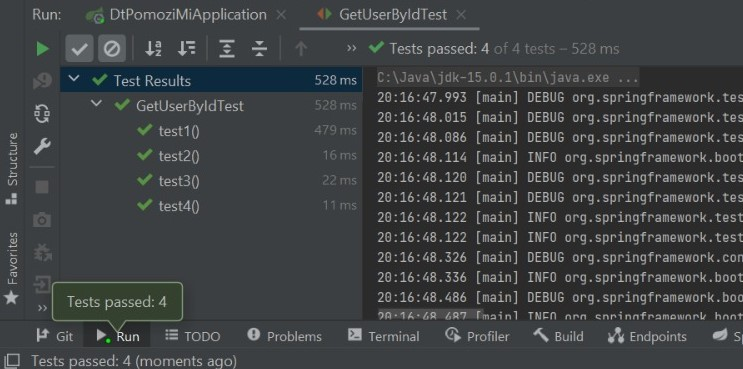
\includegraphics[width=\textwidth, height=\textheight, keepaspectratio]{slike/GetUserByIdTest.jpeg}
                \centering
                \caption{GetUserByIdTest()}
            \end{figure}
            
            \noindent \textbf{Kod unit testa: }
            \begin{verbatim}
            package NULL.DTPomoziMi.service.impl;

import static org.junit.jupiter.api.Assertions.assertEquals;
import static org.junit.jupiter.api.Assertions.assertNull;
import static org.junit.jupiter.api.Assertions.assertThrows;

import org.junit.jupiter.api.Test;
import org.springframework.beans.factory.annotation.Autowired;
import org.springframework.boot.test.context.SpringBootTest;
import org.springframework.security.authentication.
AuthenticationCredentialsNotFoundException;
import org.springframework.security.test.context.support.WithUserDetails;
import org.springframework.test.context.ActiveProfiles;

import NULL.DTPomoziMi.exception.EntityMissingException;
import NULL.DTPomoziMi.security.UserPrincipal;
import NULL.DTPomoziMi.service.UserService;
import NULL.DTPomoziMi.util.UserPrincipalGetter;

@SpringBootTest
@ActiveProfiles("dev")
class GetUserByIdTest {

	@Autowired
	private UserService service;

	private UserPrincipal principal;

	//dobar id
	@Test
	@WithUserDetails(value = "jan.rocek@gmail.com",
	userDetailsServiceBeanName = "myUserDetailsService")
	public void test1() {
		principal = UserPrincipalGetter.getPrincipal();
		assertEquals("jan.rocek@gmail.com", service.getUserByID(3, principal).getEmail());
	}

	//nepostojeci id
	@Test
	@WithUserDetails(value = "jan.rocek@gmail.com",
	userDetailsServiceBeanName = "myUserDetailsService")
	public void test2() {
		principal = UserPrincipalGetter.getPrincipal();
		assertThrows(EntityMissingException.class, 
		() -> service.getUserByID(110l, principal));
	}

	// ne-adminski dohvat tuđeg profila rezultira skrivanjem lokacije
	@Test
	@WithUserDetails(value = "matea.lipovac@gmail.com",
	userDetailsServiceBeanName = "myUserDetailsService")
	public void test3() { principal = UserPrincipalGetter.getPrincipal();
	assertNull(service.getUserByID(7, principal).getLocation()); }

	//neprijavljen korisnik
	@Test
	public void test4() { assertThrows(AuthenticationCredentialsNotFoundException.class, 
	() -> service.getUserByID(110l, principal)); }

}
            \end{verbatim}
            
            \noindent \textbf{Ispitni sličaj 5: Testiranje funkcionalnosti metode fetch()}\\
			
			\medskip
            \noindent\textbf{Ulaz:}
            \begin{packed_enum}
            \item Id korisnika kojeg se dohvaća
            \end{packed_enum}
            
            \noindent\textbf{Očekivani rezultat:}
            \begin{packed_enum}
            \item korisnik s traženim idom
            \item pripadajuća pogreška
            \end{packed_enum}
            
            \noindent \text
            Rezultat: Očekivani rezultat je zadovoljen, aplikacija je prošla sve testove \\
            
            \begin{figure}[H]
                 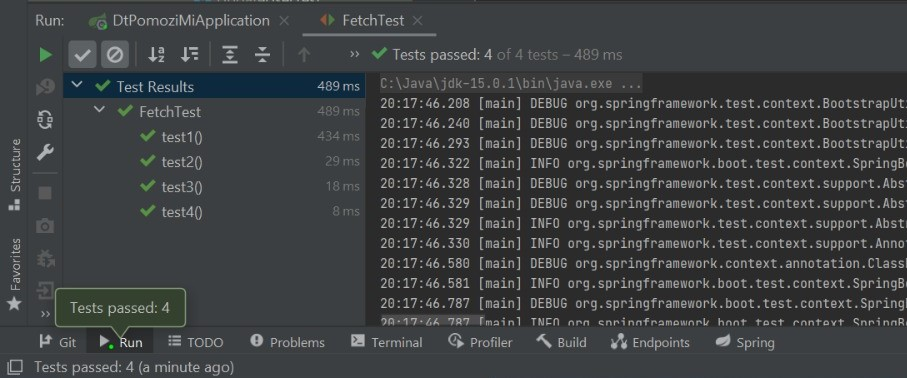
\includegraphics[width=\textwidth, height=\textheight, keepaspectratio]{slike/FetchTest.jpeg}
                \centering
                \caption{FetchTest()}
            \end{figure}
            
            \noindent \textbf{Kod unit testa: }
            \begin{verbatim}
            package NULL.DTPomoziMi.service.impl;

import static org.junit.jupiter.api.Assertions.assertEquals;
import static org.junit.jupiter.api.Assertions.assertThrows;

import org.junit.jupiter.api.Test;
import org.springframework.beans.factory.annotation.Autowired;
import org.springframework.boot.test.context.SpringBootTest;
import org.springframework.security.authentication.
AuthenticationCredentialsNotFoundException;
import org.springframework.security.test.context.support.WithUserDetails;
import org.springframework.test.context.ActiveProfiles;

import NULL.DTPomoziMi.exception.EntityMissingException;
import NULL.DTPomoziMi.repository.UserRepo;
import NULL.DTPomoziMi.security.UserPrincipal;
import NULL.DTPomoziMi.service.UserService;
import NULL.DTPomoziMi.util.UserPrincipalGetter;

@SpringBootTest
@ActiveProfiles("dev")
public class FetchTest {

	@Autowired
	private UserService service;

	@Autowired
	private UserRepo userRepo;

	//dohvat samog sebe
	@Test
	@WithUserDetails(value = "jan.rocek@gmail.com",
	userDetailsServiceBeanName = "myUserDetailsService")
	public void test1() {
		UserPrincipal principal = UserPrincipalGetter.getPrincipal();
		assertEquals(principal.getUser(), service.fetch(3));
	}

	//dohvat postojeceg korisnika
	@Test
	@WithUserDetails(value = "jan.rocek@gmail.com",
	userDetailsServiceBeanName = "myUserDetailsService")
	public void test2() { assertEquals(userRepo.findByEmail("matea.lipovac@gmail.com"), 
	service.fetch(12)); }

	//dohvat nepostojeceg korisnika
	@Test
	@WithUserDetails(value = "jan.rocek@gmail.com",
	userDetailsServiceBeanName = "myUserDetailsService")
	public void test3() { assertThrows(EntityMissingException.class, 
	() -> service.fetch(90)); }

	//neprijavljeni korisnik
	@Test
	public void test4() { assertThrows(AuthenticationCredentialsNotFoundException.class,
	() -> service.fetch(12)); }
}
            \end{verbatim}
            
            \medskip
			
			\noindent \textbf{Ispitni sličaj 6: Testiranje funkcionalnosti metode deleteRequest()}\\
			
			\medskip
            \noindent\textbf{Ulaz:}
            \begin{packed_enum}
            \item id zahtjeva koji se briše
            \item User principal
            \end{packed_enum}
            
            \noindent\textbf{Očekivani rezultat:}
            \begin{packed_enum}
            \item zahtjev sa statusom obrisan (deleted)
            \item pripadajuća pogreška
            \end{packed_enum}
            
            \noindent \text
            Rezultat: Očekivani rezultat je zadovoljen, aplikacija je prošla sve testove \\
            
            \begin{figure}[H]
                 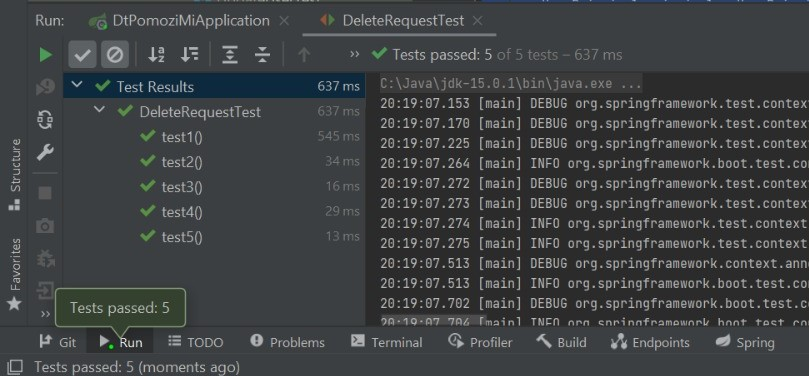
\includegraphics[width=\textwidth, height=\textheight, keepaspectratio]{slike/DeleteRequestTest.jpeg}
                \centering
                \caption{DeleteRequestTest()}
            \end{figure}
            
            \noindent \textbf{Kod unit testa: }
            \begin{verbatim}
            
            package NULL.DTPomoziMi.service.impl;

import static org.junit.jupiter.api.Assertions.assertEquals;
import static org.junit.jupiter.api.Assertions.assertThrows;

import org.junit.jupiter.api.Test;
import org.springframework.beans.factory.annotation.Autowired;
import org.springframework.boot.test.context.SpringBootTest;
import org.springframework.security.authentication.
AuthenticationCredentialsNotFoundException;
import org.springframework.security.test.context.support.WithUserDetails;
import org.springframework.test.context.ActiveProfiles;

import NULL.DTPomoziMi.exception.EntityMissingException;
import NULL.DTPomoziMi.exception.IllegalAccessException;
import NULL.DTPomoziMi.exception.IllegalActionException;
import NULL.DTPomoziMi.model.RequestStatus;
import NULL.DTPomoziMi.security.UserPrincipal;
import NULL.DTPomoziMi.util.UserPrincipalGetter;

@SpringBootTest
@ActiveProfiles("dev")
public class DeleteRequestTest {

	@Autowired
	private RequestServiceImpl service;

	//brisanje vlastitog aktivnog zahtjeva
	@Test
	@WithUserDetails(value = "matea.lipovac@gmail.com",
	userDetailsServiceBeanName = "myUserDetailsService")
	public void test1() {
		UserPrincipal principal = UserPrincipalGetter.getPrincipal();

		assertEquals(RequestStatus.DELETED,
		service.deleteRequest(35, principal).getStatus());
		assertThrows(EntityMissingException.class, () -> { service.fetch(35); });
	}

	//admin brise zahtjev
	@Test
	@WithUserDetails(value = "jan.rocek@gmail.com",
	userDetailsServiceBeanName = "myUserDetailsService")
	public void test2() {
		UserPrincipal principal = UserPrincipalGetter.getPrincipal();

		assertEquals(RequestStatus.DELETED,
		service.deleteRequest(11, principal).getStatus());
		assertThrows(EntityMissingException.class, () -> { service.fetch(11); });
	}

	//nevlasteno brisanje tudeg zahtjeva
	@Test
	@WithUserDetails(value = "robert.dakovic@gmail.com",
	userDetailsServiceBeanName = "myUserDetailsService")
	public void test3() {
		UserPrincipal principal = UserPrincipalGetter.getPrincipal();
		assertThrows(IllegalAccessException.class,
		() -> service.deleteRequest(25, principal).getStatus());
	}

	// zahtjev već ima izvrsitelja
	@Test
	@WithUserDetails(value = "matea.lipovac@gmail.com",
	userDetailsServiceBeanName = "myUserDetailsService")
	public void test4() {
		UserPrincipal principal = UserPrincipalGetter.getPrincipal();

		assertThrows(IllegalActionException.class, 
		() -> service.deleteRequest(34, principal).getStatus());
	}

	//neprijavljen korisnik
	@Test
	public void test5() {
		UserPrincipal principal = UserPrincipalGetter.getPrincipal();
		assertThrows(AuthenticationCredentialsNotFoundException.class, 
		() -> service.deleteRequest(6, principal).getStatus());
	}
}
            \end{verbatim}
            
            \medskip
			
			\noindent \textbf{Ispitni slučaj 7: Testiranje funkcionalnosti metode blockUser()}\\
			
			\medskip
            \noindent\textbf{Ulaz:}
            \begin{packed_enum}
            \item id korisnika koji se blokira
            \item enabled status - false
            \end{packed_enum}
            
            \noindent\textbf{Očekivani rezultat:}
            \begin{packed_enum}
            \item enabled status blokiranog korisnika je false
            \item pripadajuća pogreška
            \end{packed_enum}
            
            \noindent \text
            Rezultat: Očekivani rezultat je zadovoljen, aplikacija je prošla sve testove \\
            
            \begin{figure}[H]
                 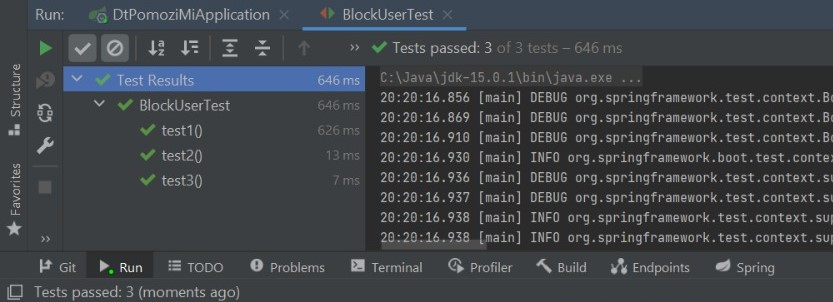
\includegraphics[width=\textwidth, height=\textheight, keepaspectratio]{slike/BlockUserTest.jpeg}
                \centering
                \caption{BlockUserTest()}
            \end{figure}
            
            \noindent \textbf{Kod unit testa: }
            \begin{verbatim}
            package NULL.DTPomoziMi.service.impl;

import static org.junit.jupiter.api.Assertions.assertEquals;
import static org.junit.jupiter.api.Assertions.assertThrows;

import org.junit.jupiter.api.Test;
import org.springframework.beans.factory.annotation.Autowired;
import org.springframework.boot.test.context.SpringBootTest;
import org.springframework.security.access.AccessDeniedException;
import org.springframework.security.authentication.
AuthenticationCredentialsNotFoundException;
import org.springframework.security.test.context.support.WithUserDetails;
import org.springframework.test.context.ActiveProfiles;

import NULL.DTPomoziMi.service.UserService;

@SpringBootTest
@ActiveProfiles("dev")
public class BlockUserTest {
	@Autowired
	private UserService service;

	// korisnik sa id=12 postoji u bazi jer se prilikom pokretanja aplikacije
	nad bazom izvode upiti 
	// uneseni u data.sql file ==> INSERT INTO korisnik (...) VALUES (12, ...)

	//admin blokira korisnika
	@Test
	@WithUserDetails(value = "jan.rocek@gmail.com",
	userDetailsServiceBeanName = "myUserDetailsService")
	public void test1() { 
	assertEquals(false,	service.blockUnblockUser(12, false).getEnabled());
	}

	//korisnik koji nije admin pokusava blokirati drugog korisnika
	@Test
	@WithUserDetails(value = "robert.dakovic@gmail.com",
	userDetailsServiceBeanName = "myUserDetailsService")
	public void test2() {
	assertThrows(AccessDeniedException.class,()->service.blockUnblockUser(12, false));
	}

	//neprijavljen korisnik
	@Test
	public void test3() {
	assertThrows(AuthenticationCredentialsNotFoundException.class, 
	() -> service.blockUnblockUser(12, false)); 
	}

}
            \end{verbatim}
            
			\subsection{Ispitivanje sustava}
			
			 \textit{Ispitivanje sustava izvedeno je koristeći radni okvir Selenium IDE kako bi se provjerila osnovna funkcionalnost
             sustava po obrascima uporabe.\\ }
			 
			 \noindent \textbf{Ispitni slučaj 1: Registracija korisnika}\\
			 \medskip
            \noindent\textbf{Ulaz:}
            \begin{packed_enum}
            \item Otvara se obrazac za registraciju
            \item Ime
            \item Prezime
            \item Email
            \item Zaporka i njena potvrda
            \item Država
            \item Mjesto
            \item Adresa
            \item Pritisak na gumb "Registracija"
            \end{packed_enum}
            
            \noindent\textbf{Očekivani rezultat:}
            \begin{packed_enum}
            \item Uspješna registracija i prikaz početne(home) stranice
            \item Pripadajuća pogreška
            \end{packed_enum}
            
            \noindent \text
            Rezultat: Očekivani rezultat je zadovoljen, aplikacija je prošla sve testove \\  
            
        \noindent \text 
        Na slici 5.8 je prikaz uspješno provedenog testa registracije u Selenium IDE.\\
        \noindent \text 
        Na slici 5.9 je prikaz obrasca prilikom neispravne registracije te pripadajuća greška.\\
		\begin{figure}[H]
                 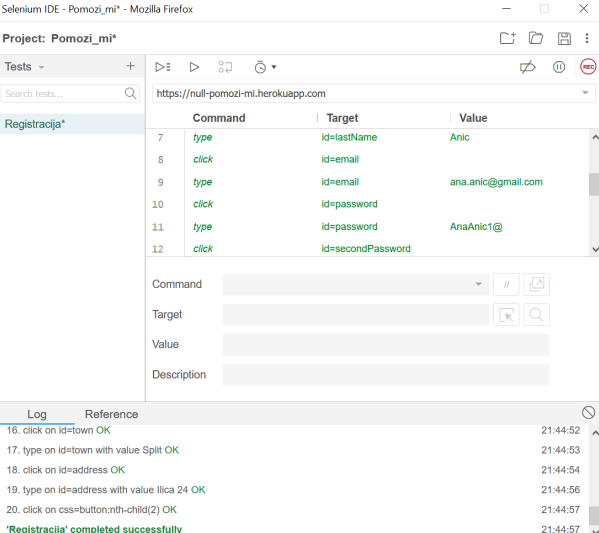
\includegraphics[width=\textwidth, height=\textheight, keepaspectratio]{slike/registracija.png}
                \centering
                \caption{Uspješan prolazak testa registracije}
        \end{figure}
		\begin{figure}[H]
                 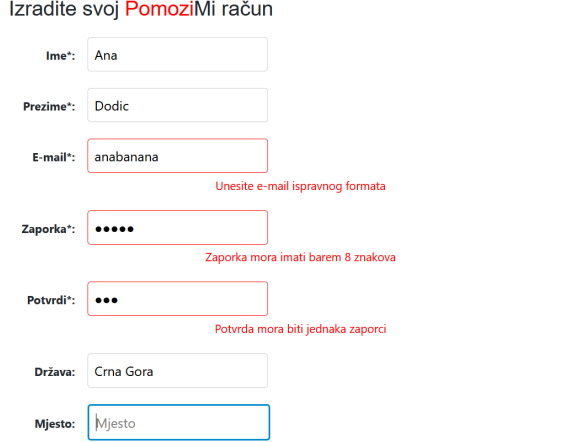
\includegraphics[width=\textwidth, height=\textheight, keepaspectratio]{slike/kriva_reg.png}
                \centering
                \caption{Krivi unos u polja registracije}
        \end{figure}
		
		\noindent \textbf{Ispitni slučaj 2: Prijava korisnika u sustav}\\
			 \medskip
            \noindent\textbf{Ulaz:}
            \begin{packed_enum}
            \item Otvara se obrazac za prijavu
            \item Email
            \item Lozinka
            \item Pritisak na gumb "Prijavi se"
            \end{packed_enum}
            
            \noindent\textbf{Očekivani rezultat:}
            \begin{packed_enum}
            \item Prikazuje se obrazac za prijavu korisnika u sustav
            \item Nakon uspješne prijave prikaz glavne stranice
            \end{packed_enum}
            
            \noindent \text
            Rezultat: Očekivani rezultat je zadovoljen, aplikacija je prošla sve testove \\  
            
        \noindent \text 
        Na slici 5.10 vidi se obrazac za prijavu korisika u sustav, a na slici 5.11 kako u Seleniumu IDE prolazi test za uspješnu prijavu.\\
		\begin{figure}[H]
                 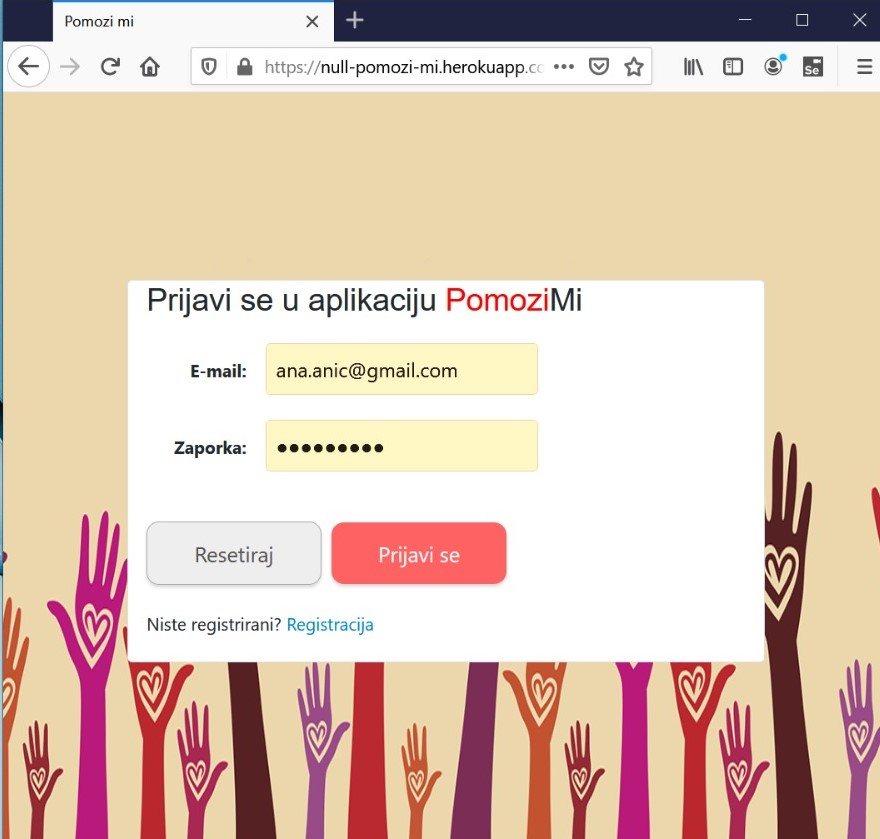
\includegraphics[width=\textwidth, height=\textheight, keepaspectratio]{slike/prijavaObrazac.jpg}
                \centering
                \caption{Prijava korisnika u sustav}
        \end{figure}
		\begin{figure}[H]
                 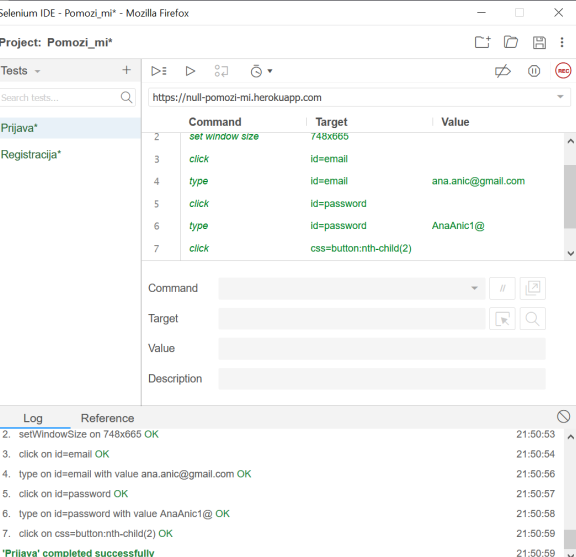
\includegraphics[width=\textwidth, height=\textheight, keepaspectratio]{slike/prijava.png}
                \centering
                \caption{Uspješan prolazak testa prijave}
        \end{figure}
			\noindent \textbf{Ispitni slučaj 3: Zadavanje zahtjeva}\\
			 \medskip
            \noindent\textbf{Ulaz:}
            \begin{packed_enum}
            \item Na izborniku odabrati "Zadavanje zahtjeva"
            \item Unos broja mobitela
            \item Unos opisa zahtjeva
            \item Lokacija : Drzava, mjesto adresa ili odabir na karti
            \item Spremanje podataka
            \item Odjava iz aplikacije
            \end{packed_enum}
            
            \noindent\textbf{Očekivani rezultat:}
            \begin{packed_enum}
            \item Prikazuje se obrazac za zadavanje zahtjeva za pomoć
            \item Opcionalni prikaz karte za lokaciju
            \item Nakon uspješnog unosa podataka, pritisak na gumb "Pošalji zahtjev"
            \end{packed_enum}
            
            \noindent \text
            Rezultat: Očekivani rezultat je zadovoljen, aplikacija je prošla sve testove \\  
            
        \noindent \text 
        Na slici 5.12 vidi se kako u Seleniumu IDE prolazi test za uspješnu prijavu, a na slici 5.13 obrazac za zadavanje zahtjeva. \\
		\begin{figure}[H]
                 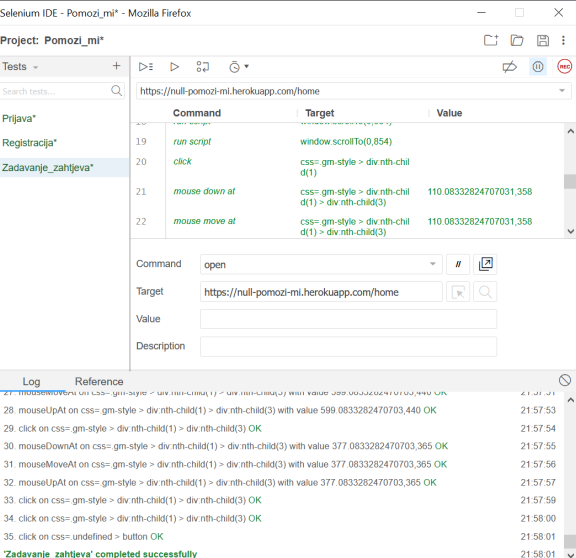
\includegraphics[width=\textwidth, height=\textheight, keepaspectratio]{slike/zadavanjeUspjesno.png}
                \centering
                \caption{Uspješan prolazak testa zadavanja zahtjeva}
        \end{figure}
		\begin{figure}[H]
                 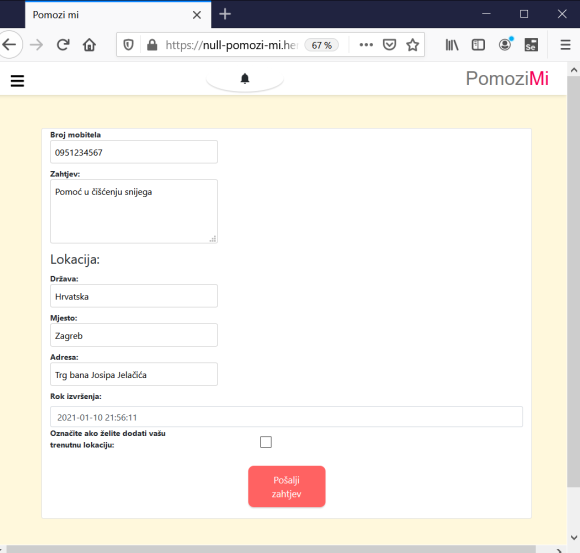
\includegraphics[width=\textwidth, height=\textheight, keepaspectratio]{slike/zadavanjeZahtjeva.png}
                \centering
                \caption{Obrazac zadavanja zahtjeva za pomoć}
        \end{figure}
        \noindent \textbf{Ispitni slučaj 4: Odabir zahtjeva za izvršavanje}\\
			 \medskip
            \noindent\textbf{Ulaz:}
            \begin{packed_enum}
            \item  Na izborniku odabrati "Pregled zahtjeva"
            \item Opcionalno unos radijusa za filtraciju
            \item Odabir gumba "izvrši zahtjev"
            \end{packed_enum}
            
            \noindent\textbf{Očekivani rezultat:}
            \begin{packed_enum}
            \item Prikazuje se izbornik na početnoj stranici
            \item Prikaz  liste aktivnih zahtjeva
            \item Opcionalni prikaz zahtjeva za unešeni radijus
            \item Nakon odabira izvršavanja šalje se notifikacija autoru
            \end{packed_enum}
            
            \noindent \text
            Rezultat: Očekivani rezultat je zadovoljen, aplikacija je prošla sve testove \\  
            
        \noindent \text 
        Na slici 5.14 vidi se kako u Seleniumu IDE prolazi test za uspješan odabir izršavanja zahtjeva, a na slici 5.15 prikaz liste aktivnih zahtjeva koje se pritiskom na gumb"Izvrši zahtijev" može odabrati za izvršavanje. \\
		\begin{figure}[H]
                 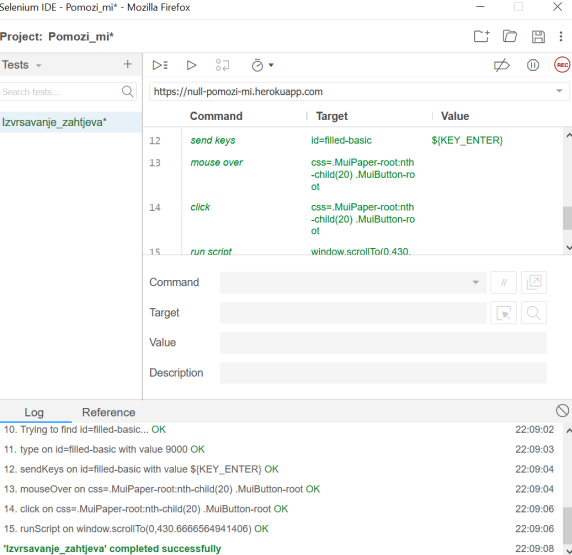
\includegraphics[width=\textwidth, height=\textheight, keepaspectratio]{slike/izvrsavanjeZahtjeva.png}
                \centering
                \caption{Uspješan prolazak testa izvršavanja zahtjeva}
        \end{figure}
		\begin{figure}[H]
                 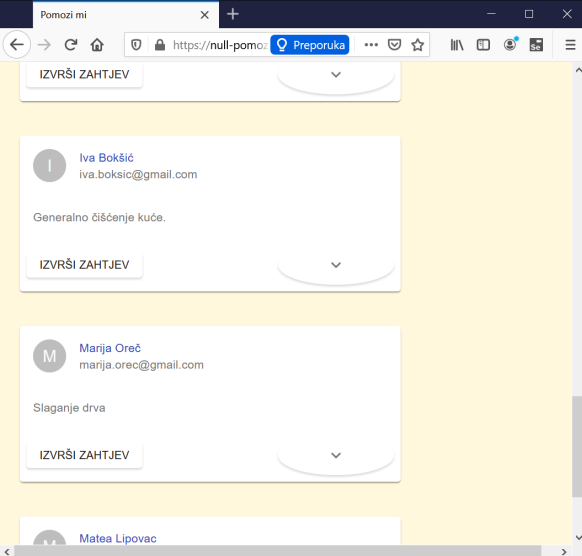
\includegraphics[width=\textwidth, height=\textheight, keepaspectratio]{slike/izvrsiZahtj.png}
                \centering
                \caption{Prikaz liste aktivnih zahtjeva}
        \end{figure}
        
        \noindent \textbf{Ispitni slučaj 5: Ocjenjivanje korisnika}\\
			 \medskip
            \noindent\textbf{Ulaz:}
            \begin{packed_enum}
            \item  Na izborniku odabrati "Korisnici"
            \item Kliknuti na ime tražene osobe
            \item Na profilu korsnika stisnuti gumb za ocjenjivanje  4. odabrati ocijena 5. stisnuti gumb "ocijeni"
            \end{packed_enum}
            
            \noindent\textbf{Očekivani rezultat:}
            \begin{packed_enum}
            \item Prikazuje se izbornik na početnoj stranici
            \item Prikaz  liste korisnika
            \item Nakon odabira imena prikaz profila
            \item Mogućnost ocijenjivanja 
            \end{packed_enum}
            
            \noindent \text
            Rezultat: Očekivani rezultat je zadovoljen, aplikacija je prošla sve testove \\  
            
        \noindent \text 
        Na slici 5.14 vidi se kako u Seleniumu IDE prolazi test za ocjenjivanje drugog korisnika, a na slici 5.15 prikaz obrasca za ocjenjivanje. \\
		\begin{figure}[H]
                 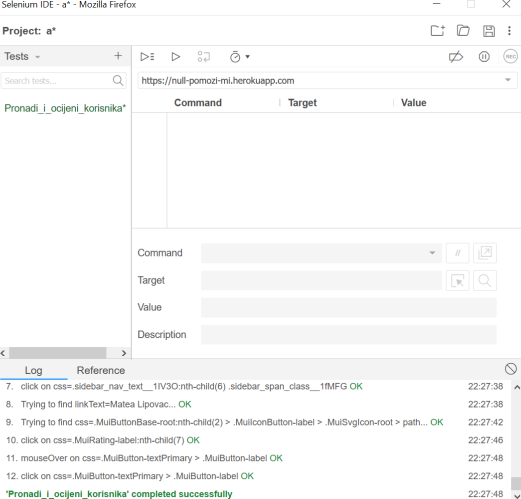
\includegraphics[width=\textwidth, height=\textheight, keepaspectratio]{slike/ocjenjivanjeSel.png}
                \centering
                \caption{Uspješan prolazak testa ocjenjivanja korisnika}
        \end{figure}
		\begin{figure}[H]
                 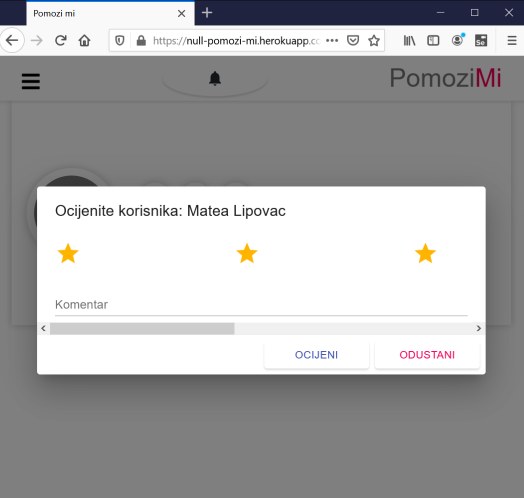
\includegraphics[width=\textwidth, height=\textheight, keepaspectratio]{slike/ocjena.png}
                \centering
                \caption{Obrazac za ocjenjivanje}
        \end{figure}
			\eject 
%\end{comment}
\section{Dijagram razmještaja}
	

	
	\text Dijagrami razmještaja opisuju topologiju sklopovlja i programsku potporu koja se koristi u implementaciji sustava u njegovom radnom okruženju. Na poslužitelju
	(HerokuCloudServer) je postavljen Linux operacijski sustav te se na njemu nalaze HTTP Server i poslužitelj baze podataka . Klijenti koriste web preglednik na svom uređaju(PC ili mobitel) kako bi pristupili web aplikaciji.Sustav je baziran na arhitekturi ”klijent – poslužitelj”, a komunikacija izmedu računala korisnika (klijent, zaposlenik,vlasnik, administrator) i poslužitelja odvija se preko HTTP veze.  

    %unos slike
		\begin{figure}[H]
			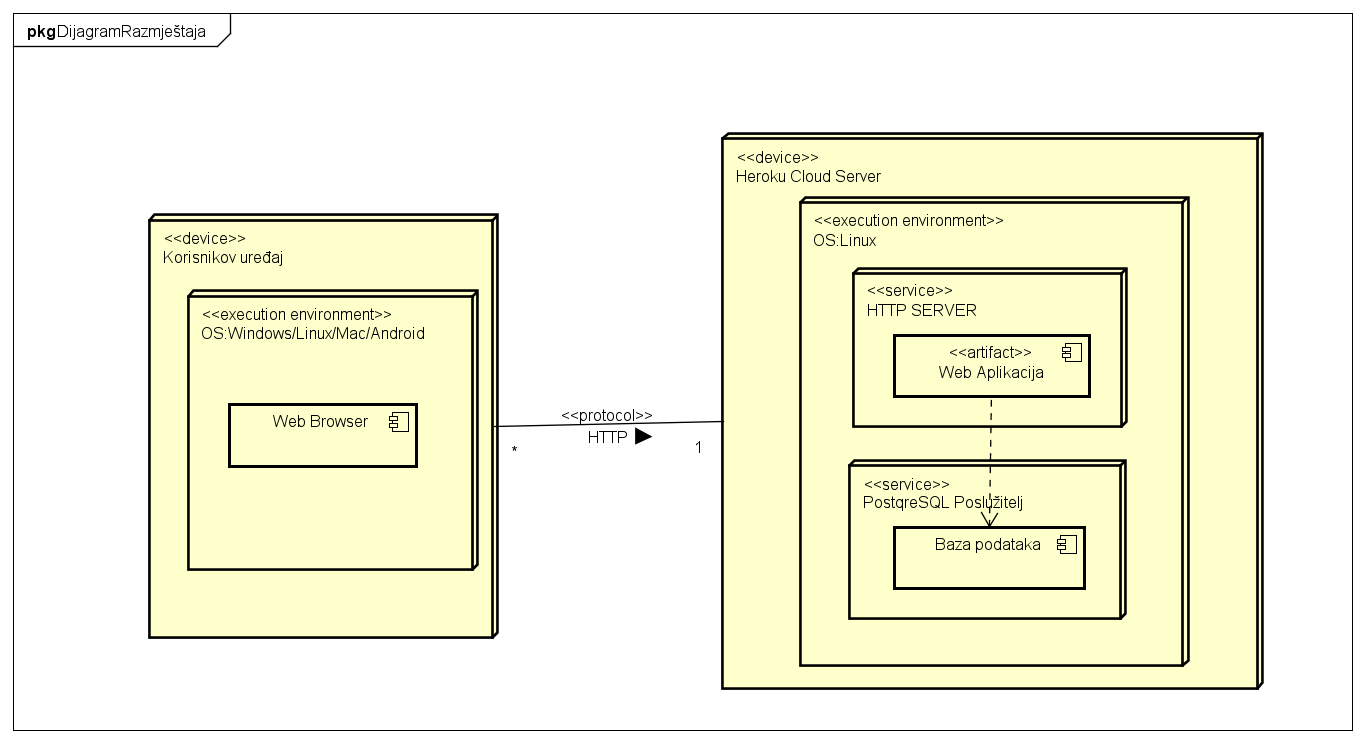
\includegraphics[scale=0.5]{slike/Dijagram Razmjestaja.png} %veličina slike u odnosu na originalnu datoteku i pozicija slike
			\centering
			\caption { Dijagram Razmještaja}
			\label{fig:5.1}
			\end{figure}


\begin{comment}	
	\textit{Potrebno je umetnuti \textbf{specifikacijski} dijagram razmještaja i opisati ga. Moguće je umjesto specifikacijskog dijagrama razmještaja umetnuti dijagram razmještaja instanci, pod uvjetom da taj dijagram bolje opisuje neki važniji dio sustava.}
	
	\eject 
\end{comment}

\newpage


\section{Upute za puštanje u pogon}


\begin{comment}
	\textit{U ovom poglavlju potrebno je dati upute za puštanje u pogon (engl. deployment) ostvarene aplikacije. Na primjer, za web aplikacije, opisati postupak kojim se od izvornog kôda dolazi do potpuno postavljene baze podataka i poslužitelja koji odgovara na upite korisnika. Za mobilnu aplikaciju, postupak kojim se aplikacija izgradi, te postavi na neku od trgovina. Za stolnu (engl. desktop) aplikaciju, postupak kojim se aplikacija instalira na računalo. Ukoliko mobilne i stolne aplikacije komuniciraju s poslužiteljem i/ili bazom podataka, opisati i postupak njihovog postavljanja. Pri izradi uputa preporučuje se \textbf{naglasiti korake instalacije uporabom natuknica} te koristiti što je više moguće \textbf{slike ekrana} (engl. screenshots) kako bi upute bile jasne i jednostavne za slijediti.}
		
		
	\textit{Dovršenu aplikaciju potrebno je pokrenuti na javno dostupnom poslužitelju. Studentima se preporuča korištenje neke od sljedećih besplatnih usluga: \href{https://aws.amazon.com/}{Amazon AWS}, \href{https://azure.microsoft.com/en-us/}{Microsoft Azure} ili \href{https://www.heroku.com/}{Heroku}. Mobilne aplikacije trebaju biti objavljene na F-Droid, Google Play ili Amazon App trgovini.}
	
	
	\eject 
\end{comment}
